\subsection{Cosine Similarity}

The cosine similarity is a measure between two vectors that is often used in documents research.

\subsubsection{The formula}

As the measure computes the similarity between two documents,  we will use $d(C_i,C_{i'} = 1 - cosine similarity$ to have a distance. In each subset $C_i$ of the corpus, we can denote $f_{i,j}$ the frequency of the word $w_j$. It is computed as follows:
\begin{eqnarray}
 d(C_i,C_{i'}) = 1 - \frac{\sum_j f_{i,j}\cdot f_{i',j}}{\sqrt{\sum_j f_{i,j}^2} \sqrt{\sum_j f_{i',j}^2 }}
\end{eqnarray}

The term $f_{i,j}$ can also be replaced by the TF-IDF term.

\subsubsection{Computations on the corpus}

We applied the cosine distance on the years contained in the corpus, producing the following matrices:

\begin{figure}[H]
    \begin{minipage}[b]{0.48\linewidth}
        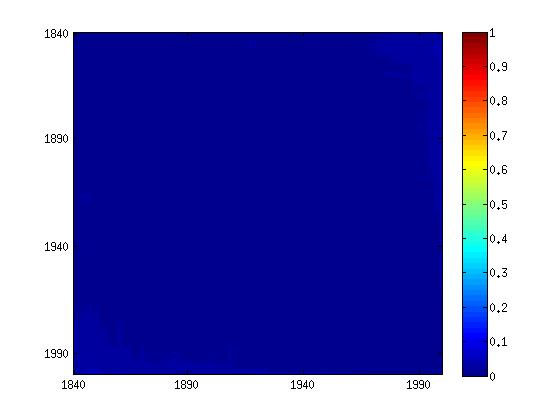
\includegraphics[scale=0.3]{Pictures/cos/cos_corrected2.jpg}
        \caption{cosine distance for 1-gram with OCR correction}
        \label{cos_1}
    \end{minipage}\hfill
    \begin{minipage}[b]{0.5\linewidth}
        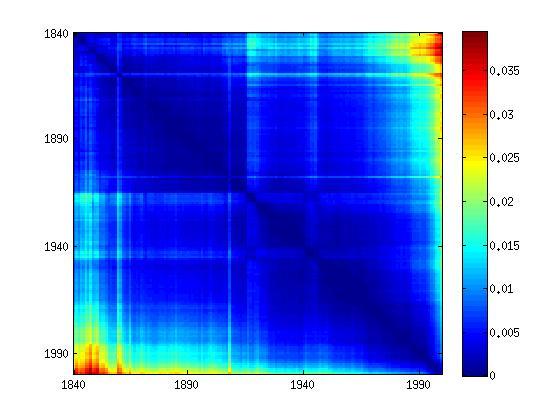
\includegraphics[scale=0.3]{Pictures/cos/cos_corrected.jpg}
        \caption{cosine distance with reduced scale on corrected corpus}
        \label{cos_2}
    \end{minipage}\hfill
\end{figure}
\begin{figure}[H]
    \begin{minipage}[b]{0.48\linewidth}
        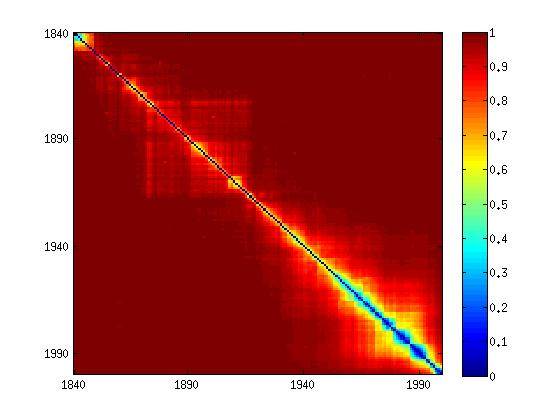
\includegraphics[scale=0.3]{Pictures/cos/cos_corrected_tfidf.jpg}
        \caption{cosine distance weighted by TF-IDF}
        \label{cos_tfidf}
    \end{minipage}\hfill
    \begin{minipage}[b]{0.48\linewidth}
        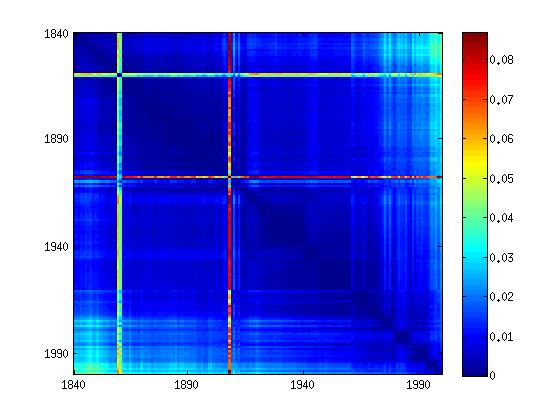
\includegraphics[scale=0.3]{Pictures/cos/cos_wo_corr.jpg}
        \caption{cosine distance on the corpus without correction}
        \label{cos_wo_corr}
    \end{minipage}\hfill
\end{figure}

\subsubsection{Analysis}

In the same manner as with the chi-square distance, this measure is usually used to compare documents and not a huge set of articles, containing a lot of common words. But in the rescaled matrix in figure \ref{cos_2}, we begin to have a more suited behaviour for our purpose. Indeed, it is smooth in the way that consecutive years have almost the same colour while there is a kind of band around the diagonal and a higher distance in the upper right and top left corners.

With the TF-IDF terms in figure \ref{cos_tfidf}, it is like if the values where all brought closer to the diagonal. We can see that 10 consecutive years look similar with each other and that the years after are much farther. It is not as smooth as expected for a good distance but it can be very useful and precise for dating.

In figure \ref{cos_wo_corr}, we can see the result of the cosine distance applied on the original OCR, without any correction. The red and yellow lines suggest that the OCR correction is well done. It shows also that some particular years are affected a lot by OCR oddities.